\documentclass[a4paper, 11pt]{article}
\pagestyle{empty}

\usepackage{ngerman}
\usepackage{nicefrac}
\usepackage{py_uebungen}

\author{Rebecca Breu}
\title{Einf"uhrung in Python --- "Ubung 1}
\date{Juni 2010}

\begin{document}
\maketitle\thispagestyle{empty}

\setlength{\fboxsep}{4mm}
\begin{center}
\fbox{\parbox{8cm}{\centering
\begin{tabular}{r@{: }l}
Login&\texttt{XXXloginXXX}\\
Passwort&\texttt{XXXpasswortXXX}
\end{tabular}\\[2mm]
Bitte das Passwort "andern (\texttt{passwd})!\\[2mm]
Editoren: kate, kwrite, emacs, gvim, gedit, jedit, eric
}}
\end{center}


\section{Datentypen I}

\begin{frame}[fragile]
\frametitle{Numerische Datentypen}
\begin{itemize}
\item \texttt{int}: entspricht \texttt{long} in C
\item \texttt{long}: unbegrenzter Wertebereich
\item \texttt{float}: enspricht \texttt{double} in C 
\item \texttt{complex}: komplexe Zahlen
\end{itemize} 
\begin{lstlisting}[style=Python]
a = 1
b = 1L
c = 1.0; c = 1e0
d = 1 + 0j
\end{lstlisting}
\vspace{3mm}
Integers werden bei Bedarf automatisch in long umgewandelt! 
\end{frame}

\begin{frame}
\frametitle{Operatoren auf Zahlen}
\begin{itemize}
\item Grundrechenarten: \texttt{+}, \texttt{-}, \texttt{*}, \texttt{/}
\item Div- und Modulo-Operator: \texttt{//}, \hspace{1mm}\texttt{\%}, \hspace{1mm}\texttt{divmod(x, y)}
\item Betrag: \texttt{abs(x)}
\item Runden: \texttt{round(x)}
\item Konvertierung: \texttt{int(x)}, \texttt{long(x)}, \texttt{float(x)}, \texttt{complex(re~[, im=0])}
\item Konjugierte einer komplexen Zahl: \texttt{x.conjugate()}
\item Potenzen: \texttt{x ** y}, \hspace{1mm}\texttt{pow(x, y)}
\end{itemize}
Ergebnis einer Verkn"upfung unterschiedlicher Datentypen ist vom Typ des \glqq gr"o"seren\grqq \, Datentyps.
\end{frame}

\begin{frame}[fragile]
\frametitle{Strings}
Datentyp: \texttt{str}
\begin{itemize}
\item \lstinline{s = 'spam'}, \lstinline{s = "spam"}
\item Mehrzeilige Strings: \lstinline{s = """spam"""}
\item keine Interpretation von Escape-Sequenzen: \lstinline{s = r"spam"}
\item Strings aus anderen Datentypen erzeugen: \lstinline{str(1.0)}
\end{itemize}
\begin{lstlisting}[style=Shell]
>>> print "sp\nam"
sp
am
>>> print r"sp\nam"
sp\nam
>>> s = """hallo
... welt"""
>>> print s
hallo
welt
\end{lstlisting}
\end{frame}

\begin{frame}
\frametitle{String-Methoden}
\begin{itemize}
\item Vorkommen von Substrings z"ahlen: \lstinline{s.count(sub [, start[, end]])}
\item beginnt/endet s mit einem Substring? \lstinline{s.startswith(sub[, start[, end]])}, \lstinline{s.endswith(sub[, start[, end]])}
\item s in Gro"s-/Kleinbuchstaben: \lstinline{s.upper()}, \lstinline{s.lower()}
\item Leerraum entfernen: \lstinline{s.strip([chars])}
\item an Substrings trennen: \lstinline{s.split([sub [,maxsplit]])}
\item Position eines Substrings finden: \lstinline{s.index(sub[, start[, end]])}
\item einen Substring ersetzen: \lstinline{s.replace(old, new[, count])}
\end{itemize}
Weitere Methoden: \lstinline{help(str)}, \lstinline{dir(str)}
\end{frame}

\begin{frame}
\frametitle{Listen}
Datentyp: \texttt{list}
\begin{itemize}
\item \lstinline{s = [1, "spam", 9.0, 42]}, \lstinline{s = []}
\item Element anh"angen: \lstinline{s.append(x)}
\item um zweite Liste erweitern: \lstinline{s.extend(s2)}
\item Vorkommen eines Elements z"ahlen: \lstinline{s.count(x)}
\item Position eines Elements: \lstinline{s.index(x[, min[, max]])}
\item Element an Position einf"ugen: \lstinline{s.insert(i, x)}
\item Element an Position l"oschen und zur"uckgeben: \lstinline{\s.pop([i])}
\item Element l"oschen: \lstinline{s.remove(x)}
\item Liste umkehren: \lstinline{s.reverse()}
\item Sortieren: \lstinline{s.sort([cmp[, key[, reverse]]])}
\item Summe der Elemente: \lstinline{sum(s)}
\end{itemize}
\end{frame}

\begin{frame}
\frametitle{Operationen auf Sequenzen}
Stings und Listen haben viel gemeinsam: Sie sind \alert{Sequenzen}.
\begin{itemize}
\item Ist ein Element in s enhalten/nicht enthalen?\\
 \lstinline{x in s}, \lstinline{x not in s}
\item Sequenzen aneinanderh"angen: \lstinline{s + t}
\item Sequenzen vervielf"altigen: \lstinline{n * s}, \lstinline{s * n}
\item i-tes Element: \lstinline{s[i]}, von hinten: \lstinline{s[-i]}
\item Subsequenz: \lstinline{s[i:j]}, mit Schrittweite k: \lstinline{s[i:j:k]}
\item Subsequenz von Anfgang/bis Ende: \lstinline{s[:-2]}, \lstinline{s[2:]}, \lstinline{s[:]}
\item L"ange: \lstinline{len(s)}
\item kleinstes/gr"o"stes Element: \lstinline{min(s)}, \lstinline{max(s)}
\item Zuweisungen: \lstinline{(a, b, c) = s} \\
$\rightarrow$ \lstinline{a = s[0]}, \lstinline{b = s[1]}, \lstinline{c = s[2]}
\end{itemize}
\end{frame}

\begin{frame}[fragile]
\frametitle{Sequenzen}
\begin{itemize}
\item Auch eine Sequenz: Datentyp \alert{\texttt{tuple}}: a = (1, 2, 3)
\item Listen sind ver"anderbar
\item Strings und Tupel sind nicht ver"anderbar
\begin{itemize}
\item Keine Zuweisung \lstinline{s[i] = ...}
\item Kein Anh"angen und L"oschen von Elementen
\item Funktionen wie \texttt{upper} liefern einen neuen String zur"uck!
\end{itemize}
\end{itemize}
\begin{lstlisting}[style=Shell]
>>> s1 = "spam"
>>> s2 = s1.upper()
>>> s1
'spam'
>>> s2
'SPAM'
\end{lstlisting}
\end{frame}

\begin{frame}[fragile]
\frametitle{Referenzen}
\begin{itemize}
\item In Python ist alles eine Referenz auf ein Objekt!
\item Vorsicht bei Zuweisungen:
\end{itemize}
\begin{lstlisting}[style=Shell]
>>> s1 = [1, 2, 3, 4]
>>> s2 = s1
>>> s2[1] = 17
>>> s1
[1, 17, 3, 4]
>>> s2
[1, 17, 3, 4]
\end{lstlisting}
Flache Kopie einer Liste: \lstinline{s2 = s1[:]} oder \lstinline{s2 = list(s1)}
\end{frame}

\begin{frame}[fragile]
\frametitle{Wahrheitswerte}
Datentyp \alert{bool}: \texttt{True}, \texttt{False}

Werte, die zu \texttt{False} ausgewertet werden:
\begin{itemize}
\item \texttt{None}
\item \texttt{False}
\item \texttt{0} (in jedem numerischen Datentyp)
\item leere Strings, Listen und Tupel: \texttt{''}, \texttt{()}, \texttt{[]}
\item leere Dictionaries: \texttt{\{\}}
\item leere Sets
\end{itemize}
Andere Objekte von eingebauten Datentypen werden stets zu \texttt{True} ausgewertet!
\begin{lstlisting}[style=Shell]
>>> bool([1, 2, 3])
True
>>> bool("")
False
\end{lstlisting}
\end{frame}

%%% Local Variables: 
%%% mode: latex
%%% latex-run-command: pdflatex
%%% TeX-master: "vortrag"
%%% End: 

\section{Statements}

\begin{frame}[fragile]{Das if-Statement}
\begin{lstlisting}[style=Python]
if a == 3:
    print "Aha!"
\end{lstlisting}
\begin{itemize}
\item Bl"ocke werden durch Einr"uckung festgelegt!
\item Standard: Einr"uckung mit vier Leerzeichen
\end{itemize}
\begin{lstlisting}
if a == 3:
    print "spam"
elif a == 10:
    print "eggs"
elif a == -3:
    print "bacon"
else:
    print "something else"
\end{lstlisting}
\end{frame}

\begin{frame}[fragile]{Vergleichsoperatoren}
\begin{itemize}
\item Vergleich des Inhalts: \texttt{==}, \texttt{<}, \texttt{>}, \texttt{<=}, \texttt{>=}, \texttt{!=}
\item Vergleich der Objektidentit"at: \lstinline{a is b}, \lstinline{a is not b}\item Und/Oder-Verkn"upfung: \lstinline{a and b}, \lstinline{a or b}
\item Negation: \lstinline{not a}
\end{itemize}
\begin{lstlisting}
if not (a==b) and (c<3):
    pass
\end{lstlisting}
\end{frame}

\begin{frame}[fragile]{Conditional Expressions}
Kurze Schreibweise f"ur bedingte Zuweisung. Statt:
\begin{lstlisting}
if zahl<0:
    s = "Negativ"
else:
    s = "Positiv"
\end{lstlisting}
kann man schreiben:
\begin{lstlisting}
s = "Negativ" if zahl<0 else "Positiv"
\end{lstlisting}
\end{frame}

\begin{frame}[fragile]{for-Schleifen}
\begin{lstlisting}[style=Python]
for i in range(10):
    print i   # 0, 1, 2, 3, ..., 9

for i in range(3, 10):
   print i    # 3, 4, 5, ..., 9

for i in range(0, 10, 2):
   print i   # 0, 2, 4, ..., 8
else:
   print "Schleife komplett durchlaufen."
\end{lstlisting}
\begin{itemize}
\item Schleife vorzeitig beenden: \lstinline{break}
\item n"achster Durchlauf: \lstinline{continue}
\item \lstinline{else} wird ausgef"uhrt, wenn die Schleife nicht vorzeitig verlassen wurde
\end{itemize}
\end{frame}

\begin{frame}[fragile]
"Uber Sequenzen kann man direkt (ohne Index) iterieren:
\begin{lstlisting}[style=Python]
for item in ["spam", "eggs", "bacon"]:
    print item
\end{lstlisting}

Auch die \texttt{range}-Funktion liefert eine Liste:
\begin{lstlisting}[style=Shell]
>>> range(0, 10, 2)
[0, 2, 4, 6, 8]
\end{lstlisting}
Ben"otigt man doch Indices:
\begin{lstlisting}[style=Python]
for (i, char) in enumerate("hallo welt"):
    print i, char
\end{lstlisting}
\end{frame}

\begin{frame}[fragile]{while-Schleifen}
\begin{lstlisting}[style=Python]
while i < 10:
    i += 1
\end{lstlisting}
Auch hier k"onnen \lstinline{break} und \lstinline{continue} verwendet werden.\\[3mm]
Ersatz f"ur do-while-Schleife:
\begin{lstlisting}[style=Python]
while True:
   # wichtiger Code
   if bedingung:
       break
\end{lstlisting} 
\end{frame}


\section{Funktionen}

\begin{frame}[fragile]{Funktionen}
\begin{lstlisting}[style=Python]
def addiere(a, b):
    """Gibt die Summe von a und b zurueck."""

    summe = a + b
    return summe
\end{lstlisting}

\begin{lstlisting}[style=Shell]
>>> ergebnis = addiere(3, 5)
>>> print ergebnis
8
>>> help(addiere)
Help on function addiere in module __main__:

addiere(a, b)
    Gibt die Summe von a und b zurueck.
\end{lstlisting}
\end{frame}

\begin{frame}[fragile]{R"uckgabewerte und Parameter}
\begin{itemize}
\item Funktionen k"onnen beliebige Objekte als Parameter und R"uckgabewerte haben
\item Typen der R"uckgabewerte und Parameter sind nicht festgelegt
\item Funktionen ohne expliziten R"uckgabewert geben \lstinline{None} zur"uck
\end{itemize}
\begin{lstlisting}[style=Python]
def hallo_welt():
    print "Hallo Welt!"

a = hallo_welt()
print a
\end{lstlisting}
\begin{lstlisting}[style=Shell]
$ mein_programm.py
Hallo Welt
None
\end{lstlisting} %$
\end{frame}

\begin{frame}[fragile]{Mehrere R"uckgabewerte}
Mehrere R"uckgabewerte werden mittels Tupel oder Listen realisiert:
\begin{lstlisting}[style=Python]
def foo():
   a = 17
   b = 42
   return (a, b)

ret = foo()
(x, y) = foo()
\end{lstlisting}
\end{frame}

\begin{frame}[fragile]{Keywords und Defaultwerte}
Man kann Parameter auch in anderer Reihenfolge als definiert angeben:
\begin{lstlisting}[style=Python]
def foo(a, b, c):
    print a, b, c

foo(b=3, c=1, a="hallo")
\end{lstlisting}
Defaultwerte festlegen:
\begin{lstlisting}[style=Python]
def foo(a, b, c=1.3):
    print a, b, c

foo(1, 2)
foo(1, 17, 42)
\end{lstlisting}
\end{frame}

\begin{frame}[fragile]{Funktionen sind Objekte}
Funktionen sind Objekte und k"onnen wie solche zugewiesen und "ubergeben werden:
\begin{lstlisting}[style=Shell]
>>> a = float
>>> a(22)
22.0
\end{lstlisting}
\begin{lstlisting}[style=Shell]
>>> def foo(fkt):
...     print fkt(33)
...
>>> foo(float)
33.0
\end{lstlisting}
\end{frame}


\newpage

\section*{Input/Output}
\begin{aufgabe}[String formatting]
Start the Python interpreter.
\begin{auflistung}
\item Display \lstinline{float} numbers with a given number of positions before and after decimal point, and in exponential notation.
\item Display \lstinline{int} numbers in hexadecimal and octal notation.
\item Given a person's given name, family name, residence and age, display the data in one line, e.g.:
\begin{verbatim}
"James Kirk is 35 years old and lives in Iowa."
\end{verbatim}
\item Try more formatting possibilities: \texttt{\underline{http://docs.python.org/lib/typesseq-strings.html}}
\end{auflistung}
\end{aufgabe}

\begin{aufgabe}[Command line parameters]
Write a program which prints its name and all its command line parameters.
\end{aufgabe}

\begin{aufgabe}[Read files]
Write a program which counts the frequency of the word "spam" in a file. \hinweis{There's a useful string method!}
\end{aufgabe}

\begin{aufgabe}[Read and write files]
Write a program which reads a file, adds a line number to each of its lines and writes the ouput to a new file. Example output:
\begin{verbatim}
1. Hallo
2. Welt
\end{verbatim}

\end{aufgabe}



\section{Errors and Exceptions}

\begin{frame}[fragile]{Syntax Errors, Indentation Errors}
Errors while parsing: \alert{Program doesn't get executed}. E.g.: 
\begin{itemize}
\item Mismatched or missing parenthesis
\item Missing or misplaced semicolons, colons, commas
\item Indentation errors
\end{itemize}
\begin{lstlisting}[style=Python]
print "I'm running..."
def add(a, b)
   return a + b
\end{lstlisting}
\begin{lstlisting}[style=Shell]
$ ./add.py
  File "add.py", line 2
    def add(a, b)
                ^
SyntaxError: invalid syntax
\end{lstlisting} %$
\end{frame}

\begin{frame}[fragile]{Exceptions}
Exceptions occur at \alert{runtime}:
\begin{lstlisting}[style=Python]
import math
print "I'm running..."
math.foo()
\end{lstlisting}
\begin{lstlisting}[style=Shell]
$ ./test.py
I'm running...
Traceback (most recent call last):
  File "test.py", line 3, in ?
    math.foo()
AttributeError: 'module' object has no 
attribute 'foo'
\end{lstlisting} %$
\end{frame}

\begin{frame}[fragile]{Handling Exceptions}
\begin{lstlisting}[style=Python]
try:
    s = raw_input("Enter a number: ")
    number = float(s)
except ValueError:
    print "That's not a number!"
\end{lstlisting}
\begin{itemize}
\item \lstinline{except} block is executed when the code in the code in the \lstinline{try}-Block throws an according exception
\item afterwards, the program continues normally
\item unhandled exceptions force the program to exit.
\end{itemize}
Handling different kinds of exceptions:
\begin{lstlisting}[style=Python]
except (ValueError, TypeError, NameError):
\end{lstlisting}
\end{frame}

\begin{frame}[fragile]{Handling Exceptions}
\begin{lstlisting}[style=Python]
try:
    s = raw_input("Enter a number: ")
    number = 1/float(s)
except ValueError:
    print "That's not a number!"
except ZeroDivisionError:
    print "You can't divide by zero!"
except:
    print "Oops, what's happened?"
\end{lstlisting}
\begin{itemize}
\item Several \lstinline{except} statements for different exceptions
\item Last \lstinline{except} can be used without specifying the kind of exception: Catches all remaining exceptions
\begin{itemize}
\item Careful: Can mask unintended programming errors!
\end{itemize}
\end{itemize}
\end{frame}

\begin{frame}[fragile]{Handling Exceptions}
\begin{itemize}
\item \alert{\texttt{else}} is executed if no exception occurred
\item \alert{\texttt{finally}} is executed \alert{in any} case
\end{itemize}
\begin{lstlisting}[style=Python]
try:
    f = open("spam")
except IOError:
    print "Cannot open file"
else:
    print f.read()
    f.close()
finally:
    print "End of try."
\end{lstlisting}
\end{frame}

\begin{frame}[fragile]{Exception Objects}
Access to exception objects:
\begin{lstlisting}[style=Python]
try:
    f = open("spam")
except IOError, e:
    print e.errno, e.strerror
    print e
\end{lstlisting}
\begin{lstlisting}[style=Shell]
$ python test.py
2 No such file or directory
[Errno 2] No such file or directory: 'spam'
\end{lstlisting}%$
\end{frame}

\begin{frame}{Exceptions in Function Calls}
\begin{figure}
\centering
\only<1>
{
  \begin{tikzpicture}
  \draw [black] (0, 0.2) node {draw()};
  \draw [white, ->] (0, 0) arc(180:270:15pt) node[anchor=west] {rectangle()};
  \draw [white, ->] (1.5, -0.7) arc(180:270:15pt) 
                    -- (2.5, -1.23) node[anchor=west] {line()};
  \draw [white] (4.6, -1.23) node {Exception!};
  \draw [white, ->] (4.5, -1.0) arc(0:90:15pt) -- (2.8, -0.47);
  \draw [white, ->] (2.6, -0.3) arc(0:90:15pt) -- (0.8, 0.225);
  \end{tikzpicture}
}

\only<2>
{
  \begin{tikzpicture}
  \draw [black] (0, 0.2) node {draw()};
  \draw [black, ->] (0, 0) arc(180:270:15pt) node[anchor=west] {rectangle()};
  \draw [white, ->] (1.5, -0.7) arc(180:270:15pt) 
                    -- (2.5, -1.23) node[anchor=west] {line()};
  \draw [white] (4.6, -1.23) node {Exception!};
  \draw [white, ->] (4.5, -1.0) arc(0:90:15pt) -- (2.8, -0.47);
  \draw [white, ->] (2.6, -0.3) arc(0:90:15pt) -- (0.8, 0.225);
  \end{tikzpicture}
}

\only<3>
{
  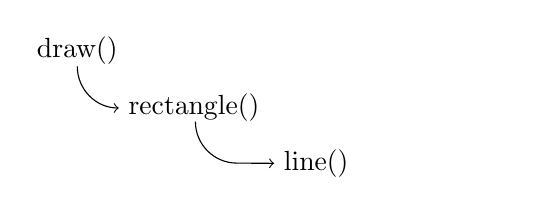
\begin{tikzpicture}
  \draw [black] (0, 0.2) node {draw()};
  \draw [black, ->] (0, 0) arc(180:270:15pt) node[anchor=west] {rectangle()};
  \draw [black, ->] (1.5, -0.7) arc(180:270:15pt) 
                    -- (2.5, -1.23) node[anchor=west] {line()};
  \draw [white] (4.6, -1.23) node {Exception!};
  \draw [white, ->] (4.5, -1.0) arc(0:90:15pt) -- (2.8, -0.47);
  \draw [white, ->] (2.6, -0.3) arc(0:90:15pt) -- (0.8, 0.225);
  \end{tikzpicture}
}

\only<4>
{
  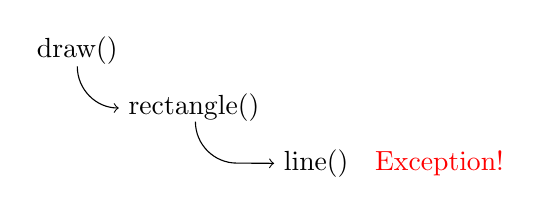
\begin{tikzpicture}
  \draw [black] (0, 0.2) node {draw()};
  \draw [black, ->] (0, 0) arc(180:270:15pt) node[anchor=west] {rectangle()};
  \draw [black, ->] (1.5, -0.7) arc(180:270:15pt) 
                    -- (2.5, -1.23) node[anchor=west] {line()};
  \draw [red] (4.6, -1.23) node {Exception!};
  \draw [white, ->] (4.5, -1.0) arc(0:90:15pt) -- (2.8, -0.47);
  \draw [white, ->] (2.6, -0.3) arc(0:90:15pt) -- (0.8, 0.225);
  \end{tikzpicture}
}

\only<5>
{
  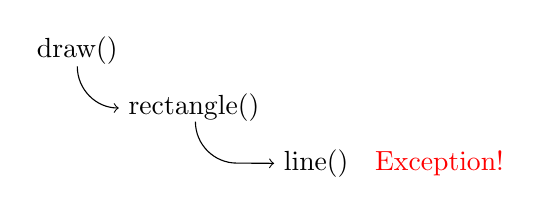
\begin{tikzpicture}
  \draw [black] (0, 0.2) node {draw()};
  \draw [black, ->] (0, 0) arc(180:270:15pt) node[anchor=west] {rectangle()};
  \draw [black, ->] (1.5, -0.7) arc(180:270:15pt) 
                    -- (2.5, -1.23) node[anchor=west] {line()};
  \draw [red] (4.6, -1.23) node {Exception!};
  \draw [white, ->] (4.5, -1.0) arc(0:90:15pt) -- (2.8, -0.47);
  \draw [white, ->] (2.6, -0.3) arc(0:90:15pt) -- (0.8, 0.225);
  \end{tikzpicture}
}

\only<6>
{
  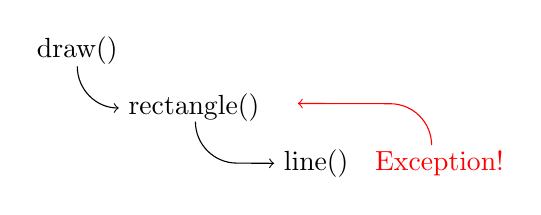
\begin{tikzpicture}
  \draw [black] (0, 0.2) node {draw()};
  \draw [black, ->] (0, 0) arc(180:270:15pt) node[anchor=west] {rectangle()};
  \draw [black, ->] (1.5, -0.7) arc(180:270:15pt) 
                    -- (2.5, -1.23) node[anchor=west] {line()};
  \draw [red] (4.6, -1.23) node {Exception!};
  \draw [red, ->] (4.5, -1.0) arc(0:90:15pt) -- (2.8, -0.47);
  \draw [white, ->] (2.6, -0.3) arc(0:90:15pt) -- (0.8, 0.225);
  \end{tikzpicture}
}

\only<7>
{
  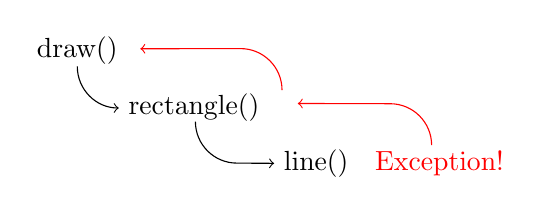
\begin{tikzpicture}
  \draw [black] (0, 0.2) node {draw()};
  \draw [black, ->] (0, 0) arc(180:270:15pt) node[anchor=west] {rectangle()};
  \draw [black, ->] (1.5, -0.7) arc(180:270:15pt) 
                    -- (2.5, -1.23) node[anchor=west] {line()};
  \draw [red] (4.6, -1.23) node {Exception!};
  \draw [red, ->] (4.5, -1.0) arc(0:90:15pt) -- (2.8, -0.47);
  \draw [red, ->] (2.6, -0.3) arc(0:90:15pt) -- (0.8, 0.225);
  \end{tikzpicture}
}
\end{figure}
\begin{itemize}
\item<1-> Function calls another function.
\item<4-> That function raises an exception.
\item<5-> Is exception handled?
\item<6-> No: Pass exception to calling function.
\end{itemize}
\end{frame}

\begin{frame}[fragile]{Raising Exceptions}
Passing exceptions on:
\begin{lstlisting}[style=Python]
try:
    f = open("spam")
except IOError:
    print "Problem while opening file!"
    raise
\end{lstlisting}
\vspace{3mm}
Raising exceptions:
\begin{lstlisting}[style=Python]
def gauss_solver(matrix):
    # Important code
    raise ValueError("Singular matrix")
\end{lstlisting}
\end{frame}


\begin{frame}[fragile]{Exceptions vs. Checking Values Beforehand}
\onslide<1->
Exceptions are preferable!

\begin{lstlisting}
def square(x):
    if type(x) == int or type(x) == float:
        return x ** 2
    else:
        return None
\end{lstlisting}
Bad!

\onslide<2->
\begin{itemize}
  \item What about other numerical data types (complex numbers, own data types)? Better: Try to compute the power and catch possible exceptions! $\rightarrow$ \alert{Duck-Typing}

  \item Caller of a function might forget to check return values for validity. Better: Raise an exception!
\end{itemize}
\end{frame}


\begin{frame}[fragile]{The \texttt{with} Statement}
Some objects offer context management, which provides a more convenient way to write \lstinline{try ... finally} blocks:
\begin{lstlisting}
with open("test.txt") as f:
    for line in f:
        print line
\end{lstlisting}
After the \lstinline{with} block the file object is guaranteed to be closed properly, no matter what exceptions occurred within the block.\vspace{5mm}

In Python 2.5 this needs the following import:
\begin{lstlisting}
from __future__ import with_statement
\end{lstlisting}
\end{frame}

\section*{Additional Excersises}

\begin{aufgabe}[High/Low]
Implement the game High/Low: A player (in this case the computer) thinks of a number between 1 and 100, the other player (in this case the user) needs to guess the number. After each try, the user is informed if his guess was too high, too low, or correct.

Proceed by the following steps:
\begin{teilaufgabe}
The program lets the user play one round and displays the number of guesses at the end of the round.
\hinweis You can create a random number between 1 and 100 by using \lstinline{random.randint(1, 100)}.
\end{teilaufgabe}
\begin{teilaufgabe}
The program asks after each round if the user wants to play again.
\end{teilaufgabe}
\begin{teilaufgabe}
The program saves a high score list in a file.
\end{teilaufgabe}

\end{aufgabe}




\vfill
\setlength{\fboxsep}{4mm}
\begin{center}
\fbox{\parbox{8cm}{\centering
War das nicht genug? Weitere Aufgaben:\\[2mm]
 \texttt{\underline{http://www.pythonchallenge.com}}
}}
\end{center}

\end{document}
